\chapter{Linear Support Vector Machines}
\label{chap:linear_svm}

In this chapter, we evaluate the performance of a Linear Support Vector Machine (SVM) on the project dataset. The primary objective is to understand how the regularization hyperparameter $C$ dictates the trade-off between margin maximization and training error, and to explore the geometric impact of data centering when computing the implicit bias term.

\section{Evaluation on Raw Data}

To train the SVM, we map the binary labels to $z_i \in \{-1, 1\}$ and apply the bias trick by appending a constant $K=1.0$ to every feature vector, yielding the augmented space $x' = [x^T, K]^T$. The model is evaluated over a logarithmic sweep of the hyperparameter $C \in [10^{-5}, 10^{0}]$.

\subsection*{Question: What do you obtain when applying the Linear SVM to the raw dataset?}

Evaluating the trained model on the evaluation set for the primary application ($\pi_T = 0.1$) yields the metrics observed in Figure \ref{fig:linear_svm_raw}. 

\begin{figure}[H]
    \centering
    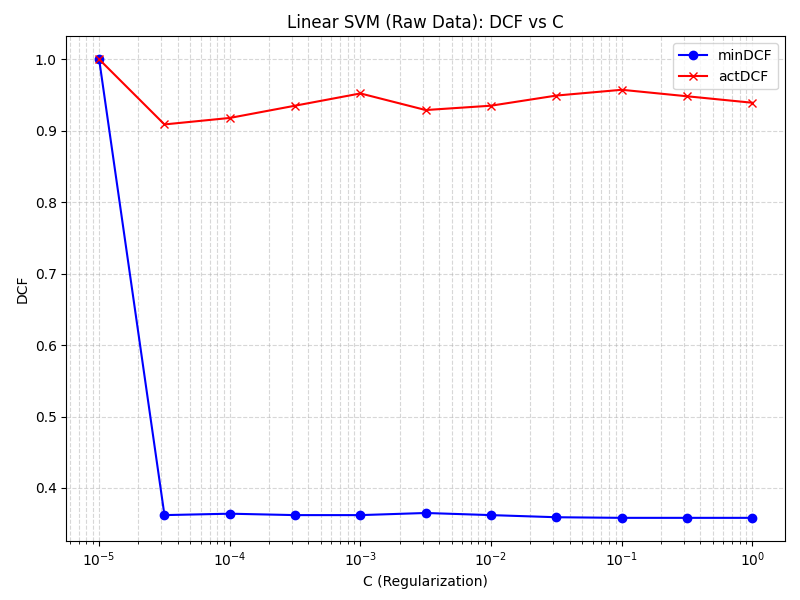
\includegraphics[width=0.85\textwidth]{Linear_SVM_Raw_DCF_vs_C.png}
    \caption{Actual DCF and Minimum DCF as a function of $C$ for the Linear SVM trained on the raw, uncentered dataset ($K=1.0, \pi_T = 0.1$).}
    \label{fig:linear_svm_raw}
\end{figure}

At extremely low values of $C$ ($10^{-5}$), the system is entirely non-informative, returning both an Actual DCF and Minimum DCF of $1.0000$. As $C$ increases toward $10^{-4}$, the discriminatory power (minDCF) improves to roughly $0.3640$. 

However, as $C$ increases further, a massive and persistent calibration gap emerges. While the Minimum DCF stabilizes at an optimal value of $0.3582$ for $C \ge 10^{-1}$, the Actual DCF remains severely degraded, plateauing around $0.9391$. 

\subsection*{Question: Can you see significant differences for the different values of C? How does the regularization coefficient affect the two metrics?}

Yes, the hyperparameter $C$ strictly dictates the performance by controlling the "softness" of the margin. It dictates the penalty applied to margin violations ($\xi_i$) in the primal objective function: $\min_{w'} \frac{1}{2}||w'||^2 + C \sum_{i=1}^n \xi_i$.

\begin{itemize}
    \item \textbf{Effect on minDCF (Ranking Ability):} When $C$ is exceptionally small (e.g., $10^{-5}$), the optimizer heavily prioritizes minimizing $||w'||^2$ to maximize the geometric margin ($M = \frac{2}{||w'||}$), largely ignoring the training data violations. The resulting hyperplane fails to separate the classes, pushing the minDCF to $1.0000$. As $C$ increases, the SVM successfully learns to separate the training samples, leading to a stabilized Minimum DCF of $0.3582$.
    \item \textbf{Effect on actDCF (Calibration):} The massive gap between minDCF and actDCF (almost $0.6$) demonstrates that while a high $C$ helps the SVM rank the samples correctly, its raw scores cannot be used directly for classification. Unlike Generative Models, the SVM score $s(x) = w^Tx + b$ represents a purely geometric distance from the margin, lacking any intrinsic probabilistic interpretation. When we evaluate the Actual DCF by comparing these geometric distances against the theoretical Bayes threshold ($t = -\log \frac{0.1}{0.9}$), the thresholding fails entirely, resulting in poor actual DCFs regardless of $C$.
\end{itemize}

\section{Evaluation on Centered Data}

In the second experiment, we compute the empirical mean of the training set ($\mu_{train}$) and subtract it from both the training and evaluation sets before training the SVM.

\subsection*{Question: What do you obtain when centering the data?}

The evaluation of the centered dataset yields the trends plotted in Figure \ref{fig:linear_svm_centered}.

\begin{figure}[H]
    \centering
    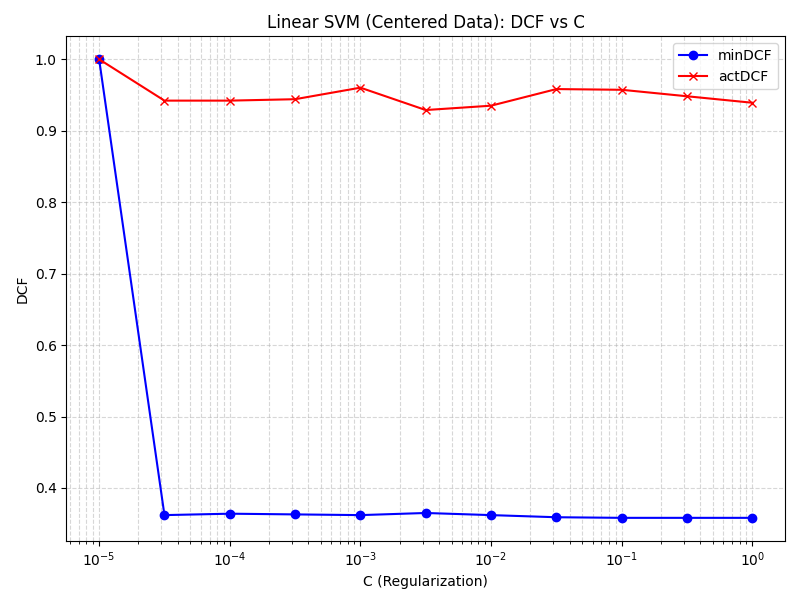
\includegraphics[width=0.85\textwidth]{Linear_SVM_Centered_DCF_vs_C.png}
    \caption{Actual DCF and Minimum DCF as a function of $C$ for the Linear SVM trained on the mean-centered dataset ($K=1.0, \pi_T = 0.1$).}
    \label{fig:linear_svm_centered}
\end{figure}

The empirical classification metrics are practically identical to those of the raw data evaluation. The optimal operating point remains in the higher $C$ range, achieving the exact same state-of-the-art Minimum DCF ($0.3582$) and Actual DCF ($0.9391$) for this linear boundary. 

\subsection*{Question: Why is data centering a fundamental pre-processing step for SVMs?}

Data centering is a theoretically vital pre-processing step due to the mechanical nature of the bias trick. When we augment the feature space by appending $K$, the implicit bias becomes $b = w_{D+1}K$. Because the SVM strictly penalizes the squared norm of the augmented weight vector ($||w'||^2 = ||w||^2 + w_{D+1}^2$), it inherently applies an artificial $L_2$ regularization penalty of $\frac{b^2}{K^2}$ to the bias term.

If the raw data is located far away from the origin, a very large bias $b$ is required to properly position the separating hyperplane. This massive $b$ incurs an extreme penalty, often forcing the optimizer to choose a sub-optimal hyperplane that sacrifices class separation simply to minimize the bias penalty. By subtracting the mean, we physically shift the mass of the data directly to the origin. The required bias $b$ becomes intrinsically small, allowing the SVM to maximize the margin based purely on the true variance of the features.

\subsection*{Question: If centering is fundamental, why are the DCF results roughly the same as the raw data?}

Even though centering is theoretically required to protect the margin from the bias penalty, it did not alter the DCF metrics in our specific experiment due to our choice of the hyperparameter $K$. 

We set $K=1.0$. The penalty applied to the bias is $\frac{b^2}{K^2}$. Because $K=1.0$ is a relatively large constant (compared to setting $K=0.01$, for instance), it provides enough "slack" in the denominator for the SVM to absorb the bias required by the raw dataset without crippling the margin penalty ($||w||^2$). Therefore, the optimizer had enough capacity to find the exact same geometric separating hyperplane in both the raw and centered spaces, resulting in identical DCFs.

However, the benefit of centering is still clearly visible in the internal optimization logs. For the centered dataset, the Primal Loss is lower and the Duality Gap is noticeably tighter compared to the raw data experiment at equivalent values of $C$. While centering did not shift the final decision boundary for this specific $K$, it drastically improved the **numerical stability and convergence** of the L-BFGS optimization algorithm.